%!TEX root = ../report.tex
\documentclass[../report.tex]{subfiles}
\usepackage{multirow}
\usepackage{threeparttable}
\usepackage{xcolor}
\usepackage{colortbl}
\usepackage{tabularx}
\usepackage{adjustbox}
\newcolumntype{M}[1]{>{\centering\arraybackslash}m{#1}}


\begin{document}
    \section{Evaluation}
    \label{sec:evaluation}

    % If your work involved experiments, describe the experimental setup and the results in this section.
    The efficiency of the simulation framework and the implemented algorithms were evaluated using a set of experiments. The experiments were performed randomly under a 
    set of different radiation source positions. The experiments were conducted in a 100x100 meter area and the drone is assumed to take off from
    the origin of the area for each test. For each source position, each algorithm is tested 10 times. Each test is considered successful if the drone is able to 
    locate a source, and the main parameters of the test will be saved into a JSON file for further analysis.  The tests under the same source position are evaluated
    together. The evaluation metrics considered for each run are prediction error, time taken to detect the source, time taken to converge the source position, 
    distance traveled by the drone to localize the source, number of iterations, and time taken for computation. The prediction error is calculated as the Euclidean
    distance between the predicted source position and the actual source position. Along with the performance metrics, the measurement history, trajectory, and computation times from each 
    iteration are also saved for further analysis. The results of the experiments are presented in the following sections.


    The tests were conducted in a 100x100 meter area with the source positioned in the following randomly selected locations: (25,80), (30,50), (50,50), (70,45), (80,70).
    \begin{figure}[ht]
        \centering
        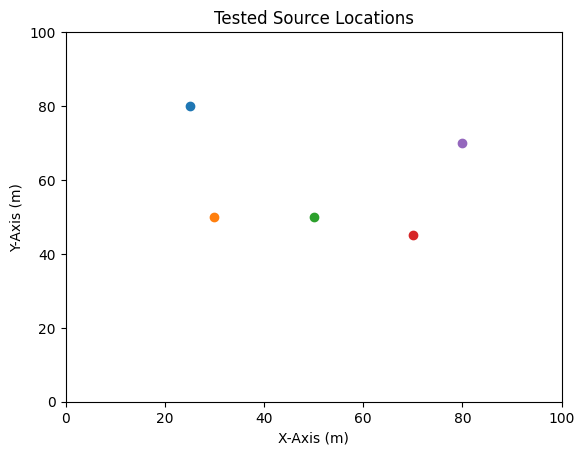
\includegraphics[width=0.8\linewidth]{figures/source_locations.png}
        \caption{Source Locations used for Evaluation}
        \label{fig:figureexample}
    \end{figure}

    \begin{table}[htbp]
        \centering
        \caption{Algorithm Performance Comparison Across Source Locations}
        \label{tab:algorithm_comparison}
        \setlength{\tabcolsep}{4pt}  % Reduce column padding (default is 6pt)
        \begin{tabular}{|c|cc|cc|cc|}
                \hline
                \multirow{2}{*}{\textbf{Location}} & \multicolumn{2}{c|}{\textbf{Entropy}} & \multicolumn{2}{c|}{\textbf{Rollout}} & \multicolumn{2}{c|}{\textbf{Inverse Square}} \\
                \cline{2-7}
                & Error (m) & Time (s) & Error (m) & Time (s) & Error (m) & Time (s) \\
                \hline
                (25, 80) & 6.01 & 125.57 & 10.24 & 177.54 & 14.38 & 415.17 \\
                \rowcolor{gray!20}
                (30, 50) & 7.06 & 43.56 & 7.00 & 108.65 & 6.62 & 470.52 \\
                (50, 50) & 7.21 & 46.12 & 6.89 & 112.45 & 6.83 & 468.24 \\
                (70, 45) & 8.17 & 45.67 & 6.66 & 115.42 & 7.71 & 415.70 \\
                (80, 70) & 8.08 & 61.85 & 6.33 & 91.62 & 4.53 & 431.01 \\
                \hline
            \end{tabular}
            \caption*{Note: Error represents prediction error in meters, Time represents convergence time in seconds}
        \end{table}
    \subsection{Analysis}

    As shown in the table~\ref{tab:algorithm_comparison}, the source location (30, 50) presents an interesting case for detailed analysis. This location was chosen for further 
    investigation because it represents the best performance across all algorithms. 
    
    
    
    \subsubsection{Prediction Error}
    \begin{figure}[ht]
        \centering
        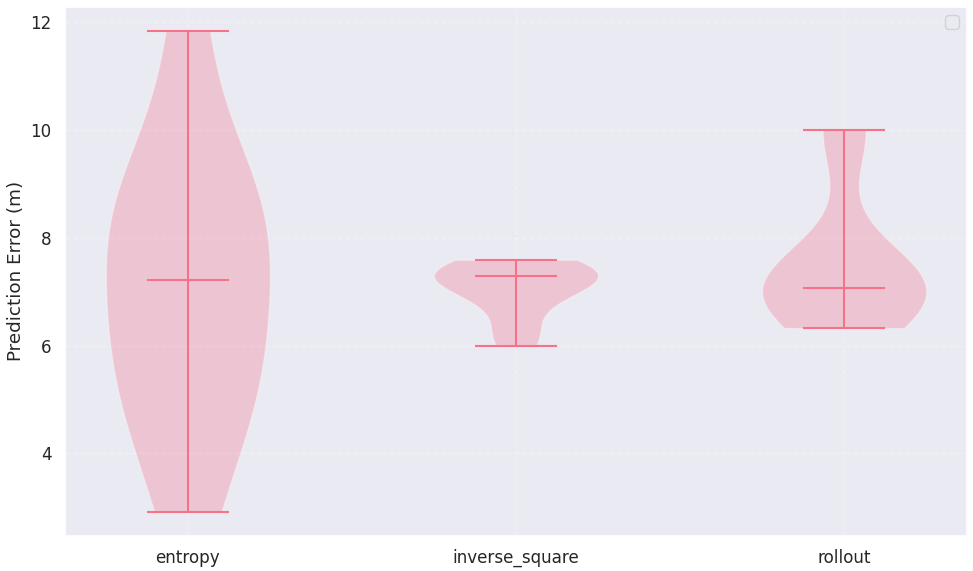
\includegraphics[width=\linewidth]{figures/prediction_violin_plot.png}
        \caption{Violin plot of prediction error for source location (30, 50)}
        \label{fig:prediction_violin_plot}
    \end{figure}

    The violin plot in Figure~\ref{fig:prediction_violin_plot} illustrates the distribution of prediction errors across all implemented algorithms. The entropy algorithm demonstrates the widest 
    range of performance, achieving both the highest (approximately 12 m) and lowest (approximately 2 m) prediction errors among all algorithms. The plot's characteristic narrowing at higher 
    error values indicates that these larger errors occur infrequently, suggesting they are outliers rather than typical performance. Notably, the algorithm's ability to achieve the lowest 
    prediction errors in some runs demonstrates its potential for high accuracy under favorable conditions.

    The median error of the entropy algorithm is approximately 7m, which aligns with findings from previous studies by Ristic et al. \cite{Ristic2007AnIG} and \cite{ristic2010information}. In 
    contrast, the inverse square algorithm exhibits a distinctly narrow spread, with errors consistently falling between 6 and 7.5 meters. This concentrated distribution of around 7 meters reflects 
    the algorithm's consistency across runs, which can be attributed to its systematic measurement collection from fixed points within the search area relative to the source location.

    The rollout algorithm shows prediction errors ranging from 6 to 10 meters, with most errors clustering around 7 meters, similar to the other algorithms. The algorithm's minimum error of 7 
    meters occurs frequently, which can be attributed to the chosen grid size (5 m) naturally leading to localization errors in the range of 5 to 7 meters. This pattern suggests that the grid 
    resolution plays a significant role in determining the algorithm's precision limits.

    \subsubsection{Convergence Time}

    \begin{figure}[ht]
        \centering
        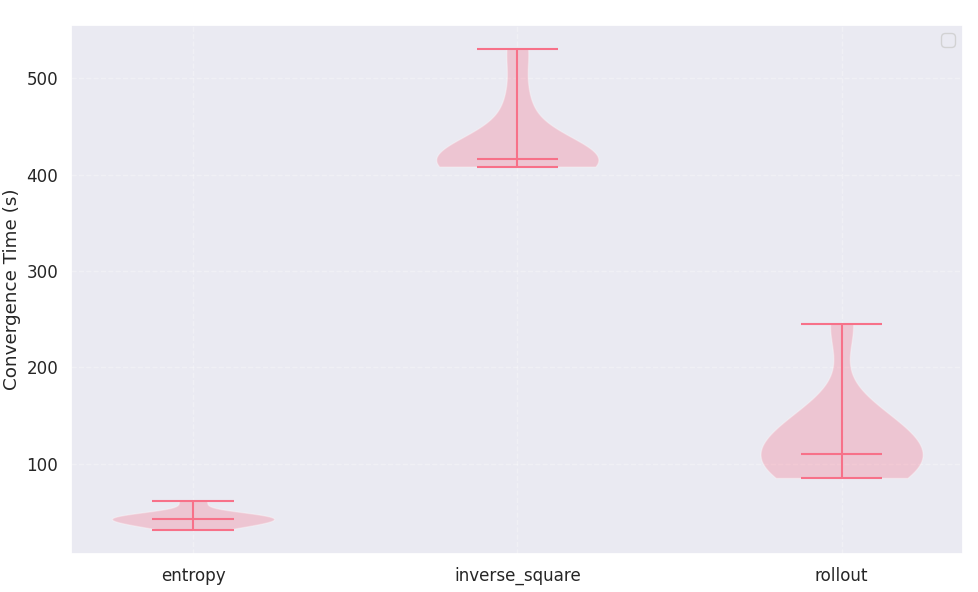
\includegraphics[width=\linewidth]{figures/convergence_violin_plot.png}
        \caption{Violin plot of convergence time for source location (30, 50)}
        \label{fig:convergence_violin_plot}
    \end{figure}

    

    \subsection{Statistical Analysis}

    Since radiation counts follow a Poisson Distribution \cite{ristic2010information}, non-parametric tests were selected for algorithm comparison. Specifically, the Wilcoxon Signed-Rank Test was 
    employed to provide detailed comparisons of paired samples, accounting for both the direction and magnitude of differences. All tests were conducted at a significance level of 0.05.

    \subsubsection{Prediction Error Analysis}
    The statistical analysis of prediction errors using the Wilcoxon Signed-Rank Test revealed no significant differences between the algorithms, with detailed results presented in Table~\ref{tab:wilcoxon_prediction_results}. These findings suggest that all three algorithms achieve comparable levels of accuracy in source localization.
    \begin{table}[ht]
        \caption{Wilcoxon Signed-Rank Test Results for Prediction Error}
        \label{tab:wilcoxon_prediction_results}
        \centering
        \begin{tabular}{|p{0.25\linewidth}|p{0.3\linewidth}|p{0.3\linewidth}|}
        \hline
        \rowcolor{gray!10} 
        Method Comparison & Statistical Results & Performance Summary \\
        \hline
        Entropy vs. Inverse Square & 
        Sample size: 10 \newline
        Statistic (W): 26.0000 \newline
        p-value: 0.9219 \newline
        Effect size (r): 0.0483 & 
        Equal performance distribution with 5 samples favoring each algorithm. Negligible effect size indicates no practical difference in accuracy. \\
        \hline
        Entropy vs. Rollout & 
        Sample size: 10 \newline
        Statistic (W): 21.0000 \newline
        p-value: 0.5566 \newline
        Effect size (r): 0.2095 & 
        Slight advantage for Entropy (6 vs 4 samples) but small effect size and non-significant p-value indicate comparable performance. \\
        \hline
        Inverse Square vs. Rollout & 
        Sample size: 10 \newline
        Statistic (W): 19.0000 \newline
        p-value: 0.4316 \newline
        Effect size (r): 0.2740 & 
        Minor advantage for Inverse Square (6 vs 4 samples) but small effect size suggests minimal practical difference. \\
        \hline
        \end{tabular}
    \end{table}



    \paragraph{Detailed Analysis}
    The pairwise comparisons revealed several key insights:
       \begin{itemize}
           \item The comparison between Entropy and Inverse Square methods showed perfect balance (5 wins each) with a negligible effect size (r = 0.0483), strongly suggesting equivalent performance.
           \item While Entropy showed a slight advantage over Rollout (6 vs 4 samples), the small effect size (r = 0.2095) and non-significant p-value (0.5566) indicate that this difference is not practically meaningful.
           \item Similarly, Inverse Square's slight advantage over Rollout (6 vs 4 samples) yielded a small effect size (r = 0.2740) and non-significant p-value (0.4316), suggesting comparable performance levels.
       \end{itemize}
   
    \vspace{0.3cm}

    \paragraph{Interpretation of Results}
    The consistency in non-significant results across all three comparisons, combined with small to negligible effect sizes, provides strong evidence that the algorithms achieve similar levels of prediction accuracy. This is particularly noteworthy given the balanced distribution of positive and negative ranks across comparisons, suggesting that any observed differences are likely due to random variation rather than systematic performance differences.
    
    \vspace{0.3cm}
    
    \subsubsection{Convergence Time Analysis}
   
    The convergence time analysis utilizing the Wilcoxon Signed-Rank Test uncovered systematic performance differences among the algorithms.
   
    \paragraph{Wilcoxon Signed-Rank Test Results}
   
    Table~\ref{tab:wilcoxon_results} presents the results of the Wilcoxon Signed-Rank Test conducted to compare the `convergence\_time` metric across the three algorithms: entropy, 
    inverse\_square, and rollout. Each pairwise comparison assessed whether there were statistically significant differences in convergence times between the algorithms.

    \begin{table}[ht]
        \caption{Wilcoxon Signed-Rank Test Results for Convergence Time}
        \label{tab:wilcoxon_results}
        \centering
        \begin{tabular}{|p{0.25\linewidth}|p{0.3\linewidth}|p{0.3\linewidth}|}
            \hline
            \rowcolor{gray!10} 
            Method Comparison & Statistical Results & Performance Summary \\
            \hline
            Entropy vs. Inverse Square & 
            Sample size: 10 \newline
            Statistic (W): 0.0000 \newline
            p-value: 0.0020 \newline
            Effect size (r): 0.8864 & 
            Complete advantage for Entropy (10 vs 0 samples) with large effect size demonstrating clear performance superiority in convergence speed. \\
            \hline
            Entropy vs. Rollout & 
            Sample size: 10 \newline
            Statistic (W): 0.0000 \newline
            p-value: 0.0020 \newline
            Effect size (r): 0.8864 & 
            Complete advantage for Entropy (10 vs 0 samples) with large effect size showing consistent superior performance in convergence time. \\
            \hline
            Inverse Square vs. Rollout & 
            Sample size: 10 \newline
            Statistic (W): 0.0000 \newline
            p-value: 0.0020 \newline
            Effect size (r): 0.8864 & 
            Complete advantage for Rollout (10 vs 0 samples) with large effect size indicating consistently faster convergence than Inverse Square. \\
        \hline
        \end{tabular}
    \end{table}

    \paragraph{Detailed Pairwise Analysis}

    The Wilcoxon Signed-Rank Test results indicate significant and substantial differences in convergence times among the three algorithms.

    Entropy consistently achieved faster convergence times than the Inverse Square method across all 10 paired samples. This difference is statistically significant (p = 0.0020) with a large 
    effect size (r = 0.8864), indicating that the observed performance improvement is both meaningful and practically significant.

    Similarly, Entropy outperformed Rollout in all 10 paired samples, demonstrating a statistically significant difference (p = 0.0020) and a large effect size (r = 0.8864). This suggests that 
    Entropy not only performs better but does so consistently across all instances tested.

    In contrast, Rollout consistently achieved faster convergence times than Inverse Square in all 10 paired samples. The results are statistically significant (p = 0.0020) with a large effect 
    size (r = 0.8864), underscoring the superior performance of Rollout over Inverse Square.

    \paragraph{Rank Summary}

    For each pairwise comparison, the rank summaries are as follows:

    In the comparison between Entropy and Inverse Square, all 10 paired samples favored Entropy, resulting in 0 positive ranks (Inverse Square performed better) and 10 negative ranks (Entropy 
    performed better), with no ties.

    Similarly, in the Entropy versus Rollout comparison, all 10 paired samples favored Entropy, leading to 0 positive ranks (Rollout performed better) and 10 negative ranks (Entropy performed 
    better), with no ties.

    Lastly, in the Inverse Square versus Rollout comparison, all 10 paired samples favored Rollout, resulting in 10 positive ranks (Rollout performed better) and 0 negative ranks (Inverse Square 
    performed better), with no ties.

    \paragraph{Interpretation of Results}

    The Wilcoxon Signed-Rank Test outcomes reveal clear and consistent performance hierarchies among the three algorithms. Entropy consistently outperforms both Inverse Square and Rollout, 
    achieving faster convergence times across all paired samples. Additionally, Rollout outperforms Inverse Square in all paired samples. These findings suggest that the Entropy algorithm is the 
    most efficient in terms of convergence time, followed by Rollout, with Inverse Square being the least efficient among the three.

    The Wilcoxon Signed-Rank Test results indicate whether the observed differences between algorithms are likely real or due to chance, based on the comparison of p-values with the significance 
    level ($\alpha$ = 0.05). The value 0.05 is commonly used for significance levels and it is the probability of rejecting the null hypothesis when it is actually true - in other words, the probability of making a Type I error (a false positive) \cite{loftus2021basic}. 

    Effect sizes ($r$) provide insight into the magnitude of the differences. Large effect sizes($r > 0.5$), as observed in all comparisons, suggest that the differences are not only statistically significant 
    but also practically meaningful for real-world applications.

\end{document}
